\section*{Supporting visualizations for internal review}
The following files retain the detailed analyses behind the shortened manuscript narrative. They are optional and are not included in the default preview.
\begin{figure*}[p]\centering
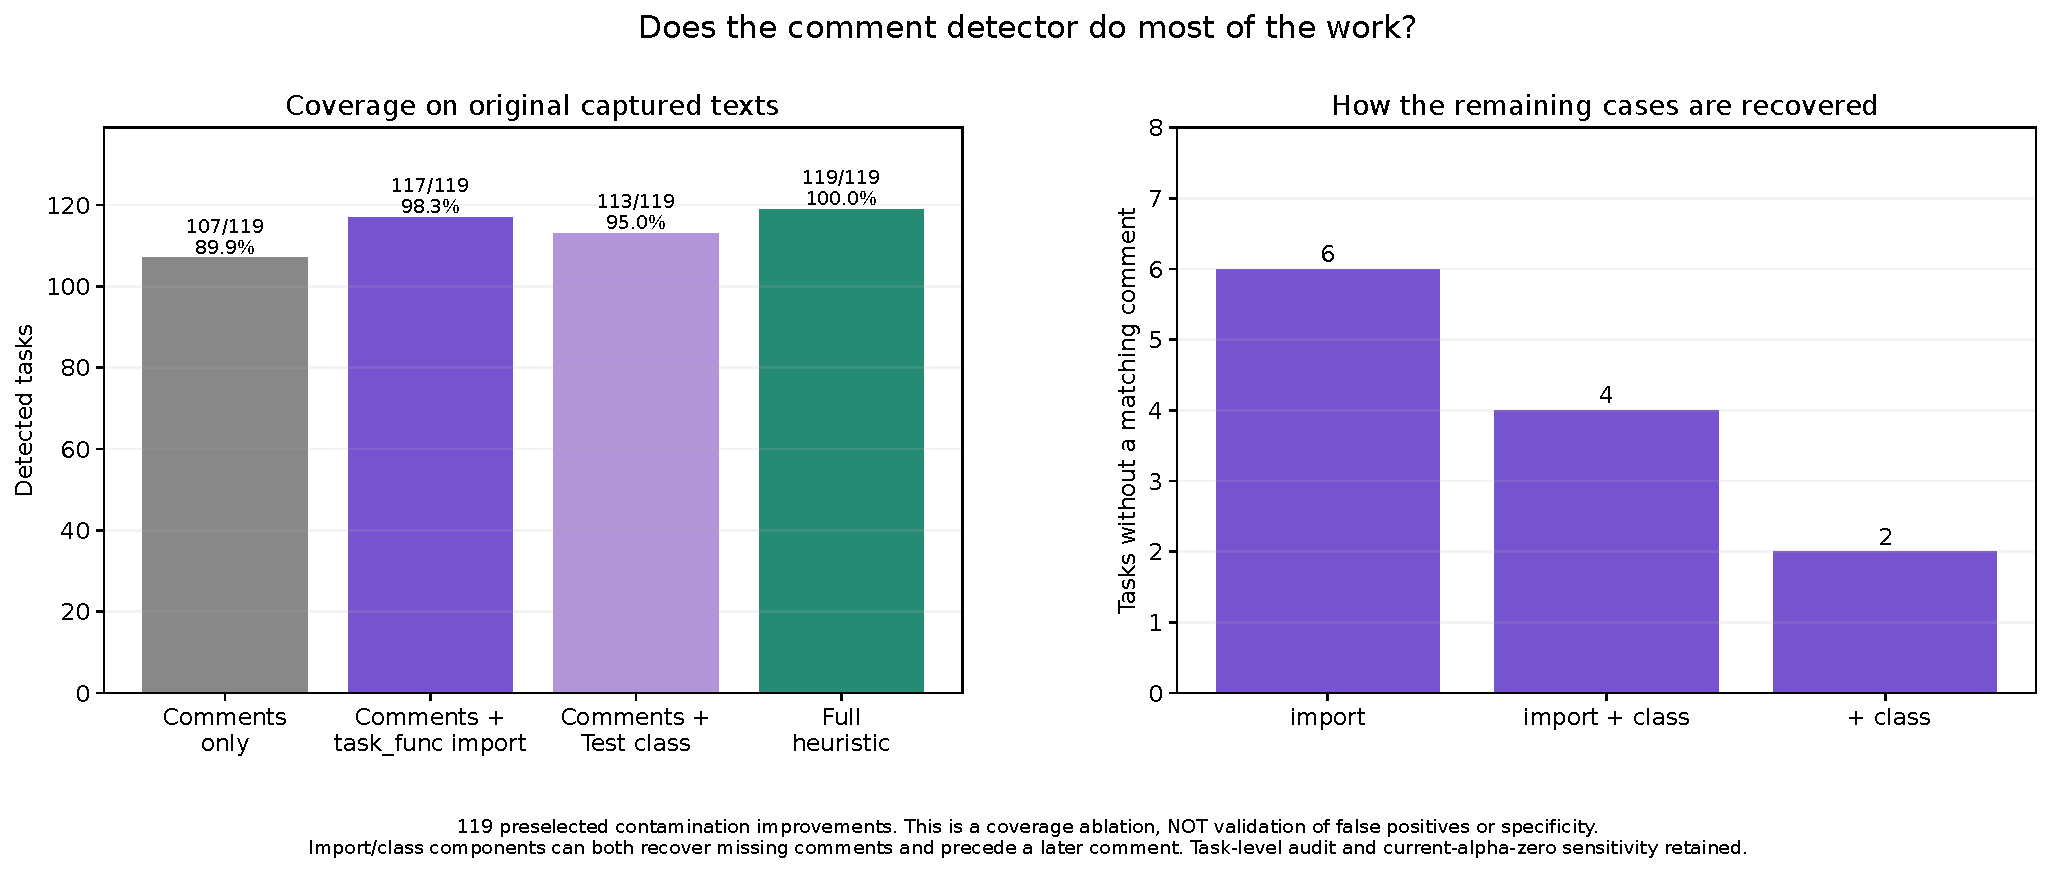
\includegraphics[width=\textwidth]{crosscoder_case_studies/supporting_figures/marker_component_ablation.pdf}
\caption{Coverage ablation of the DeepSeek lexical marker on the selected contamination cohort. Coverage is not a test of specificity on arbitrary correct programs.}
\end{figure*}
\begin{figure*}[p]\centering
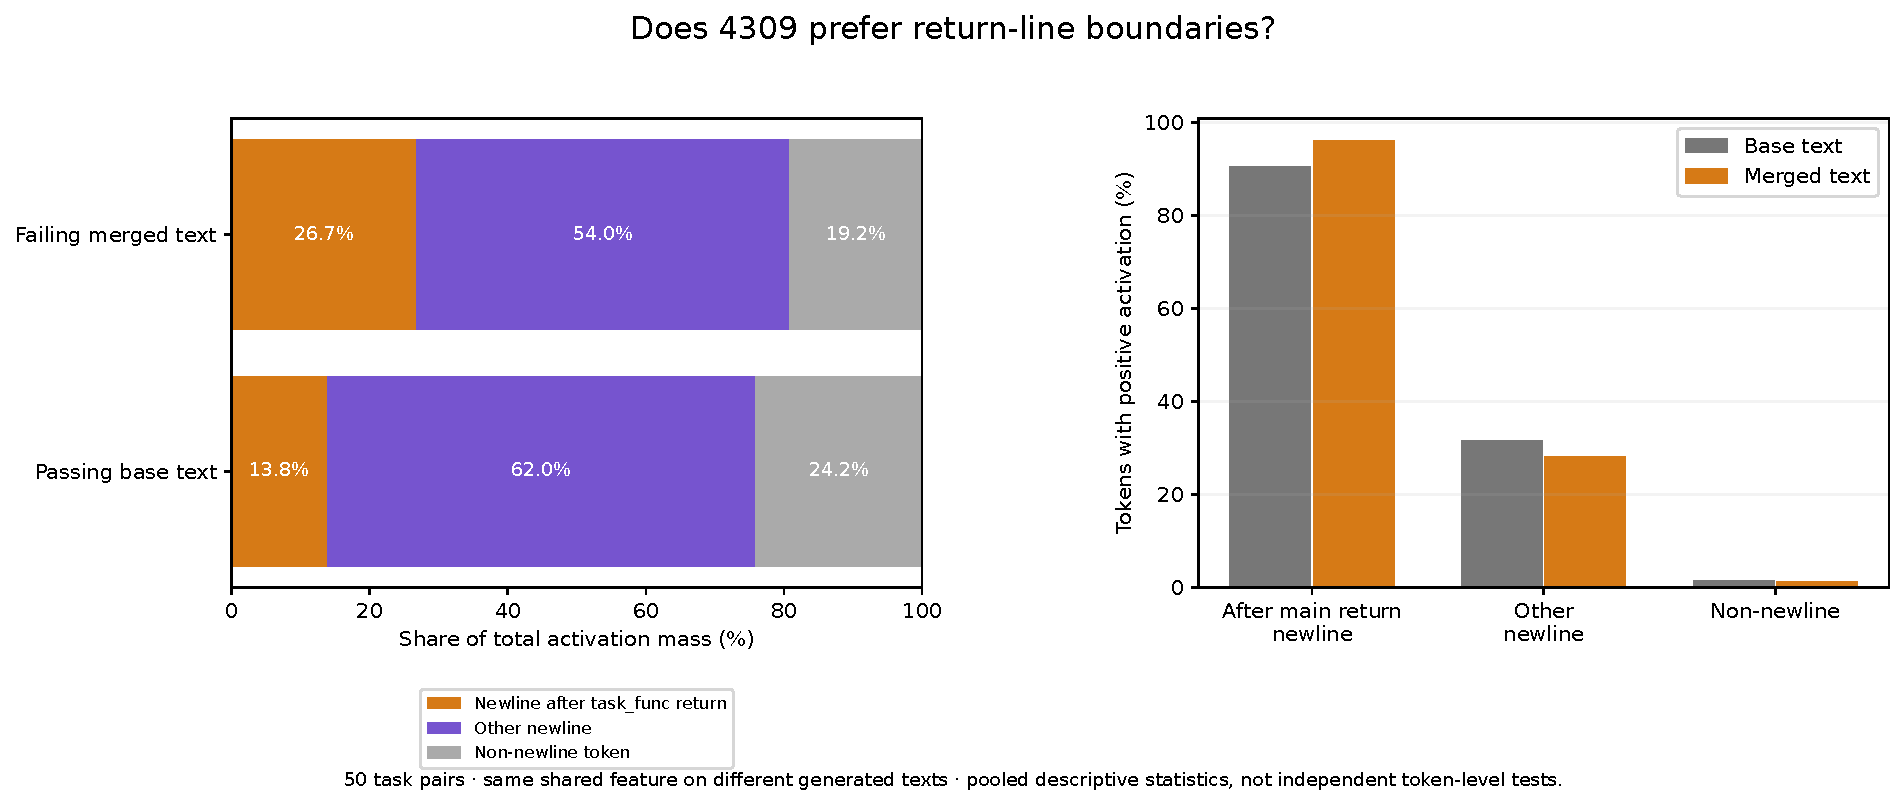
\includegraphics[width=\textwidth]{crosscoder_case_studies/supporting_figures/codellama_return_newline_specificity.pdf}
\caption{CodeLlama return-newline token statistics. Activation rate and share of activation mass are different quantities; the preference also occurs in passing base-generated texts.}
\end{figure*}
\begin{figure*}[p]\centering
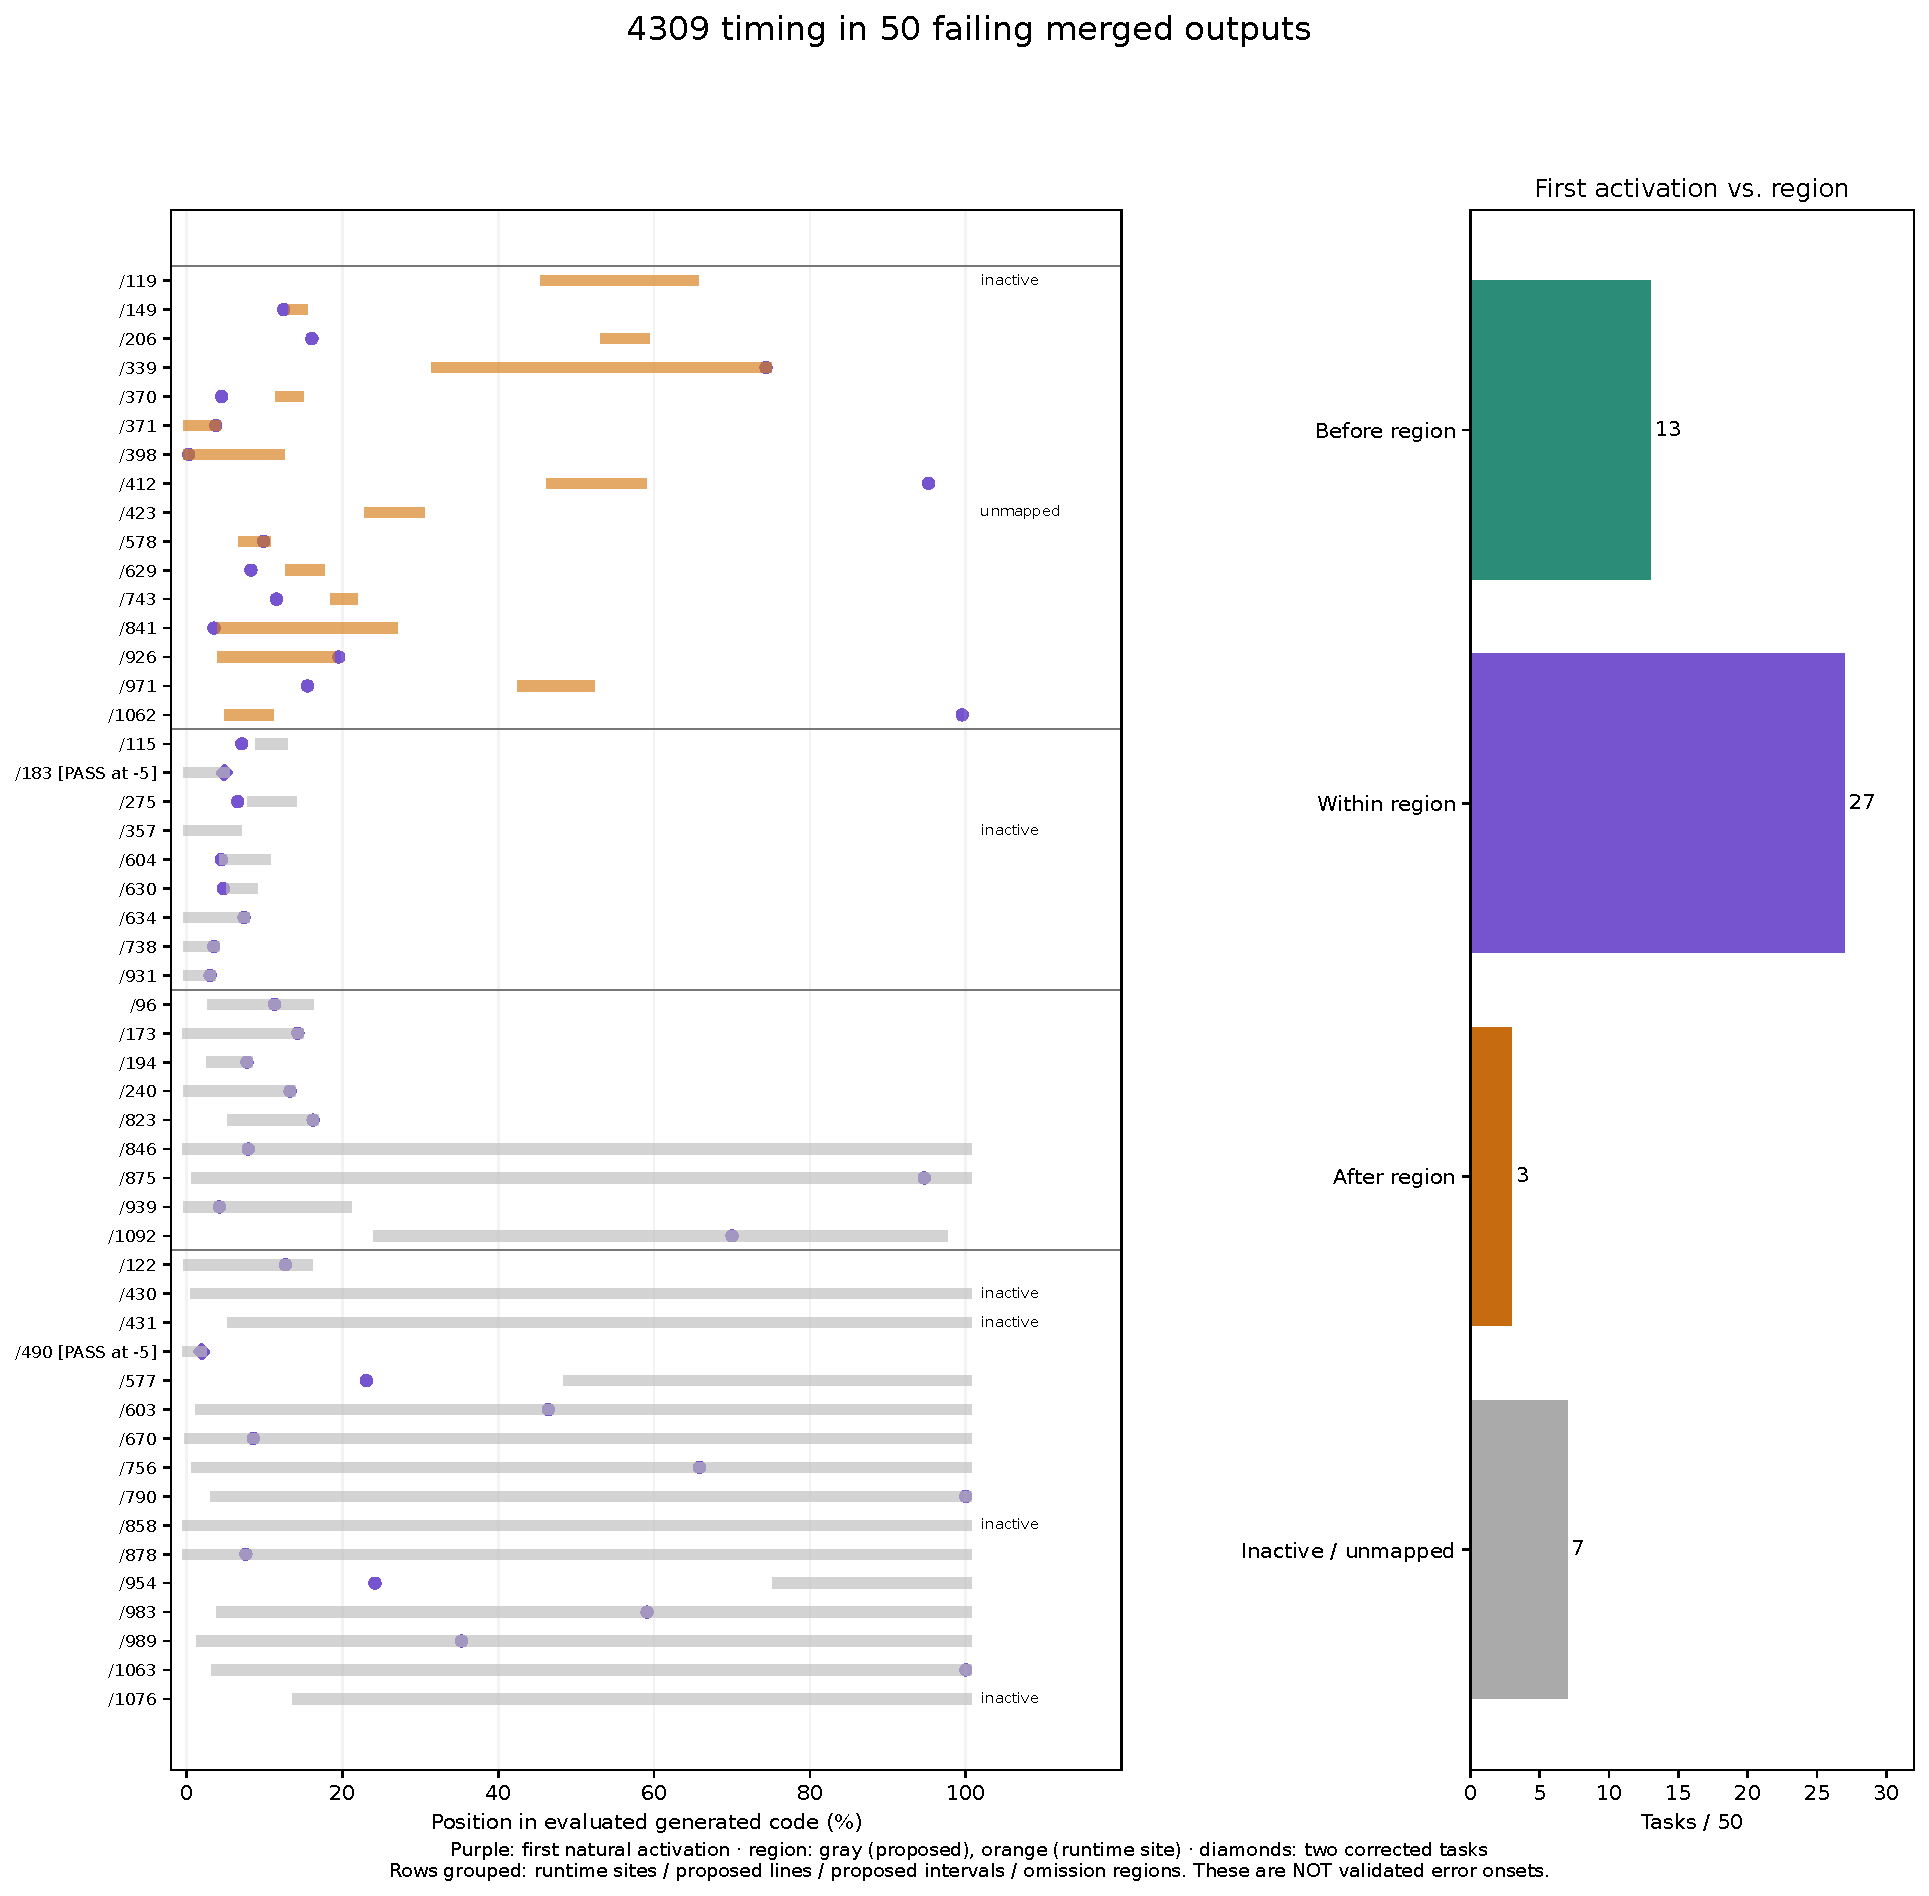
\includegraphics[height=0.84\textheight,keepaspectratio]{crosscoder_case_studies/supporting_figures/codellama_all50_regions.pdf}
\caption{All 50 CodeLlama localized regions and first mapped natural activations. Regions have different evidence tiers and are not validated earliest semantic-error onsets.}
\end{figure*}
\begin{figure*}[p]\centering
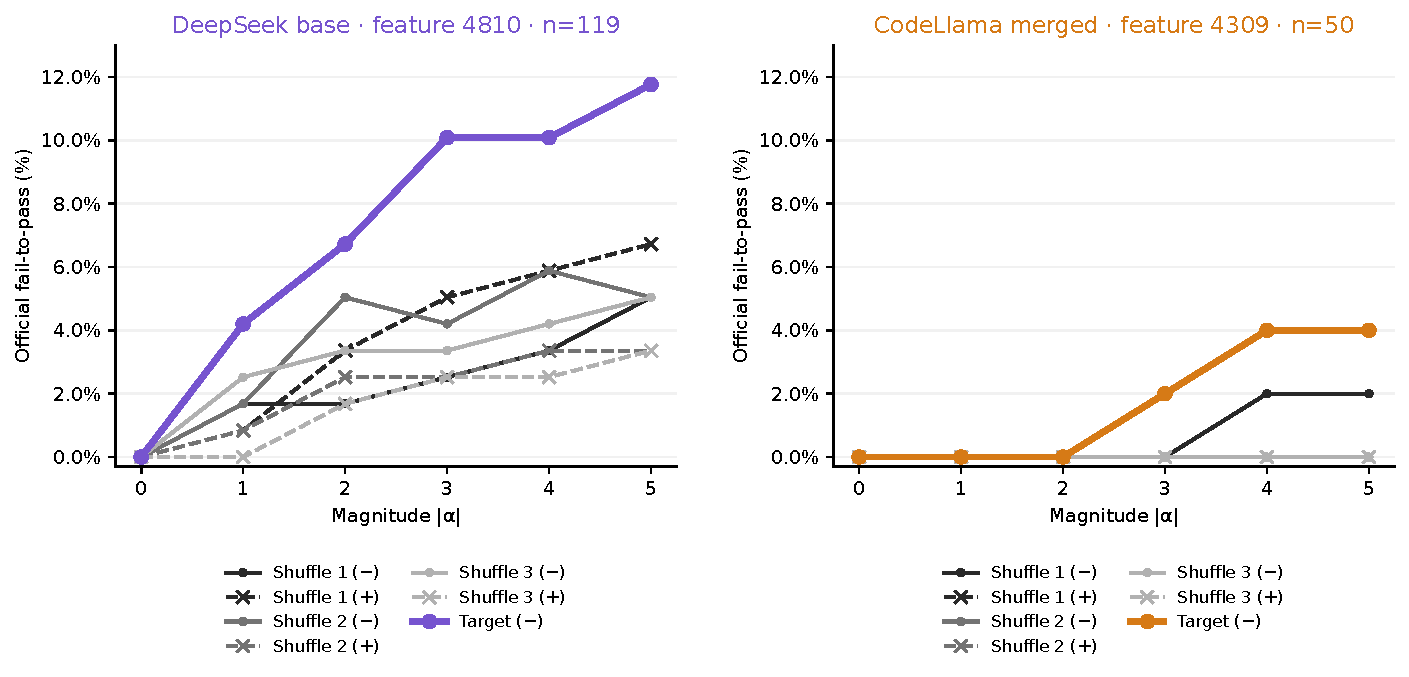
\includegraphics[width=\textwidth]{crosscoder_case_studies/supporting_figures/shuffle_both_signs.pdf}
\caption{Additional shuffled-control sign sensitivity. The main manuscript comparison uses controls in the same negative direction as both targets.}
\end{figure*}
\clearpage
